\section{Introdução}

Este documento tem como objetivo definir a arquitetura que será implementada no projeto, apontando características baseadas nas decisões anteriores, servindo como orientação para o desenvolvimento. 

\subsection{Finalidade}

Definir a estrutura arquitetural do projeto Climacolândia Doces, descrevendo os problema de forma técnica, tendo como alvo a equipe de desenvolvimento.

\subsection{Escopo}

Aplicação web que seguirá os pontos descritos neste documento, tais descritos através de diagramas de caso de uso, diagramas de classe e textos descritivos. A construção da aplicação será embasada nos tópicos descritos.

\subsection{Definições, acrônimos e abreviações}

\begin{itemize}
	\item MVT: Model -- View -- Template (inglês)
	\item MVC: Model -- View -- Controller (inglês)
	\item UC: User Case (inglês)		
\end{itemize}

\section{Representação da Arquitetura}

Será utilizado no projeto o framework Django para a linguagem de programação Python.

Por padrão, o framework Python Django utiliza o modelo arquitetural MVT, que possui três camadas: Model, View, Template. Bastante semelhante ao MVC, com a diferença nomenclatural. Uma representação gráfica da arquitetura MVT é mostrada na figura \ref{fig:mvt}

\begin{figure}[h!]
	\centering
	\includegraphics[scale=0.7]{figuras/MVT.png}
	\caption{Representação da arquitetura MVT utilizada pelo framework Django}
	\label{fig:mvt}
\end{figure}

\section{Metas e Restrições de Arquitetura}

As características estabelecidas para o Climacolândia se encontraram no documento de visão no que se refere aos requisitos não funcionais. Desta forma, visando à qualidade do sistema foram estabelecidos os seguintes critérios:

Das Metas:

\begin{itemize}
	\item Usabilidade: O sistema deve ser fácil de compreender e de ser utilizado, tanto pela parte dos clientes quanto pela parte dos mantenedores.
	\item Confiabilidade: O sistema deve ter confiabilidade, pois a gerencia de recursos e materiais da empresa estarão na aplicação, e devem estar disponíveis apenas para os mantenedores.
	\item Desempenho:	O sistema deverá estar disponível 24 horas por dia, 7 dias por semana.
	\item Manutenibilidade: O sistema deve ser construído respeitando as boas práticas de programação do framework python django, acarretando em fáceis manutenções periódicos.
	\item Portabilidade: O sistema deve ser capaz de rodar em vários navegadores pela falta de controle de qual browser a aplicação será acessada.
\end{itemize}

\section{Caso de Uso}

Os casos de uso, levantados a partir dos requisitos encontrados no documento de visão presente no anexo \ref{doc:visao}, estão presentes no diagrama mostrado na figura \ref{fig:usecase}

\begin{figure}[h!]
	\centering
	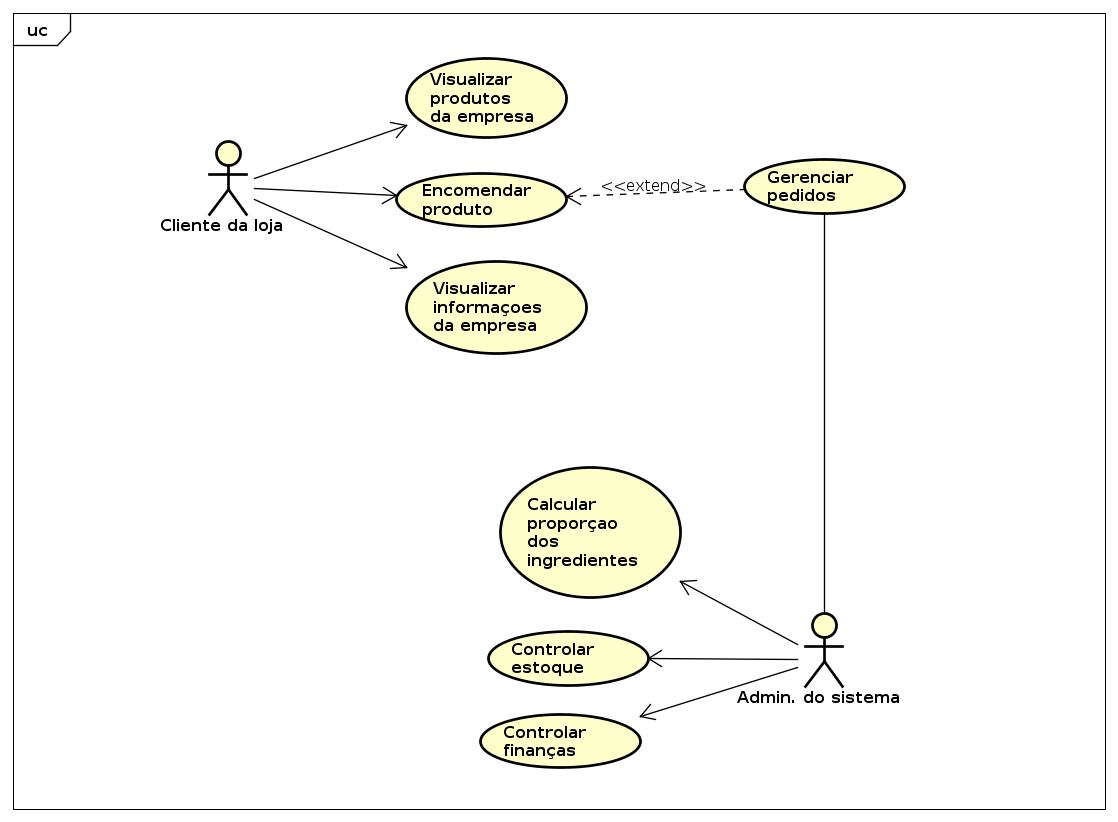
\includegraphics[scale=0.5]{figuras/usecase.png}
	\caption{Casos de uso referentes à aplicação}
	\label{fig:usecase}
\end{figure}

\subsection{Atores}

\begin{itemize}
	\item Administrador do sistema: Este ator representa as pessoas que irão realizar as funções operacionais da empresa no sistema. Estes são os mantenedores descritos no documento de visão.

	\item Cliente: Este ator representa os possíveis consumidores da empresa.
\end{itemize}

\subsection{Descrição dos Casos de Uso}

Os casos de uso estão identificados na tabela \ref{tab:usecase}

\begin{table}[!h]
\centering
\caption{Casos de uso}
\label{tab:usecase}
\resizebox{.5\textwidth}{!}{%
\begin{tabular}{|l|l|}
\hline
\rowcolor[HTML]{9B9B9B} 
Id & Caso de Uso \\ \hline
AUC01 & \cellcolor[HTML]{FFFFFF}Controlar finanças \\ \hline
AUC02 & Controlar estoque \\ \hline
AUC03 & Calcular proporção dos ingredientes \\ \hline
AUC04 & Gerenciar pedidos \\ \hline
CUC01 & Visualizar produtos da empresa \\ \hline
CUC02 & Visualizar informações da empresa \\ \hline
CUC03 & Encomendar produto \\ \hline
\end{tabular}%
}
\end{table}

\subsubsection{Descrições}

\begin{itemize}
	\item AUC01: O Administrador do Sistema deverá ser capaz de controlar os gastos, despesas e lucros da empresa
	\item AUC02: O Administrador do Sistema irá controlar o estoque, mantendo atualizadas as informações de baixas e renovação de estoque
	\item AUC03: O Administrador do sistema, irá utilizar-se da calculadora de ingredientes para obter a proporção certa dos ingredientes utilizados em alguma receita
	\item AUC04: O Administrador do sistema irá atender à demanda de pedidos realizados pelos clientes. Visualizando primeiramente, para então excluí-los ou marcando-os como concluídos
	\item CUC01: Esse caso de uso é usado pelo cliente para visualizar os produtos anteriores da empresa. Os produtos que o cliente visualiza devem ser importados da página facebook da empresa
	\item CUC02: Este caso de uso é utilizado pelo cliente para visualizar as informações da empresa Climacolandia. 
	\item CUC03: Este caso de uso é utilizado pelo cliente para fazer a encomenda de um produto. No entanto, a finalização do pedido deve ser feito diretamente com o mantenedor via telefone
\end{itemize}

\section{Visão Lógica}
\subsection{Diagrama de Pacotes}

A figura x contém a representação dos pacotes utilizados no projeto e o relacionamento entre eles

% colocar figura aqui %

\subsection{Camadas}
\subsubsection{Model}

Esta camada acessa os dados. Contendo todas as informações, validações e comportamentos que esses dados possuem.

\subsubsection{View}

Camada lógica. Acessa a camada Model, suas operações, informações, etc e os submete a camada Template.

\subsubsection{Template}

Camada  de apresentação. Contém a disposição de como algo deve ser mostrado no formato Web.

\subsubsection{Form}

Esta funciona como receptora dos dados que serão passados à view, contém os tipos de dados que cada método recebe.

\section{Tamanho e Desempenho}

Por se tratar de uma empresa com o mostruário de produtos sendo utilizado diretamente do facebook, o sistema terá uma carga significativa a menos. Sendo assim, em questão de tamanho, se trata de um sistema pequeno, visto que o mesmo comportará apenas o banco de dados do estoque e pedidos realizados dos clientes, ainda com a maior parte das operações sendo realizadas pelos administradores do sistema. Quanto ao desempenho, o sistema estará limitado à velocidade da internet em conjunto ao desempenho do navegador no dispositivo, pois trata-se de um sistema web.

\section{Qualidade}

A maior parte do sistema será privada aos administradores da Climacolândia, tendo como um dos pontos cruciais de qualidade a segurança do banco de dados, este podendo apenas ser disponível aos administradores. Se tratando dos clientes da empresa, o importante é o acesso aos trabalhos e a realização do pedido, esta que necessita que o sistema garanta a privacidade dos dados do cliente. 